\documentclass{article} % use option titlepage to get the title on a page of its own.
\usepackage{polski}
\usepackage[utf8]{inputenc}
\usepackage{graphicx}
\usepackage[a4paper, total={7in, 10in}]{geometry}
\usepackage{listings}
\usepackage{amsmath}
\usepackage[section]{placeins}
\usepackage{float}
\graphicspath{ {../plots} }
\renewcommand{\vec}[1]{\mathbf{#1}}
\newcommand{\matr}[1]{\mathbf{#1}}
\title{Metody aproksymacji interpolacyjnej}
\date{29.05.2020r}
\author{Maciej Jabłoński 175591}
\begin{document}
\maketitle

\section{Wprowadzenie}

Celem projektu było zaimplementowanie dwóch metod interpolacji - metoda wielomianowa Lagrange'a oraz metoda funkcji sklejanych, w celu zapoznania się z charakterystyką problemu interpolacji oraz zaletami i wadami poszczególnych metod.\\
Do implementacji wykorzystany został język Python i bilioteka Numpy.

\section{Interpolacja}
Interpolacja jest podzbiorem działań aproksymacyjnych. Pozwala na wyznaczenie bardzo dokładnych wartości, które znajdują się pomiędzy węzłami pomiarowymi. Różni się od ogólnej aproksymacji tym, że wyznaczone krzywe przechodzą przez podane węzły, dlatego wymogiem jest wysoka dokładność pomiaru.

\subsection{Metoda wielomianowa}
Metoda ta opiera się na twierdzeniu Weierstrassa, które mówi że dowolną funkcję \(y=f(x)\) która jest ciągła na przedziale domkniętym, można przybliżyć za pomocą wielomianu odpowiednio wysokiego stopnia. Mając \(n+1\) węzłów (punktów pomiarowych) możliwe jest rozwiązanie układu równań, którego rozwiązaniem będą współczynniki wynikowego wielomianu. W praktyce jednak okazuje się, że taki sposób prowadzi do powstania macierzy o bardzo dużych i bardzo małych wartościach, co powoduje duży błąd numeryczny, a także paradoksalnie zwiększając liczbę punktów nie zwiększamy istotnie ilości informacji o wartości funkcji.

\subsection{Metoda Lagrange'a}
Metoda Lagrange'a jest rozszerzoną wersją metody wielomianowej, w której funkcję opisujemy jako sumę pośrednich wielomianów \(\phi_i(x)\). Ogólny wzór na wielomian Lagrange'a:
\begin{equation}
    w(x) = \sum\limits_{i=0}^{n} y_i \cdot\prod\limits_{j=0 \wedge j\ne i}^n \frac{x-x_j}{x_i - x_j}
\end{equation}
Poszczególne iloczyny cechują się tym, że tylko \(i\)-ty wielomian \(\phi_i\) ma wartość niezerową w \(x_i\).
\newpage
\subsubsection{Dokładność dopasowania w zależności od liczby węzłów}
Na poniższych grafikach widnieją dopasowania wielomianów do kilku różnych zbiorów punktów pomiaru wysokości w czasie.
\begin{figure}[H]
    \centering
    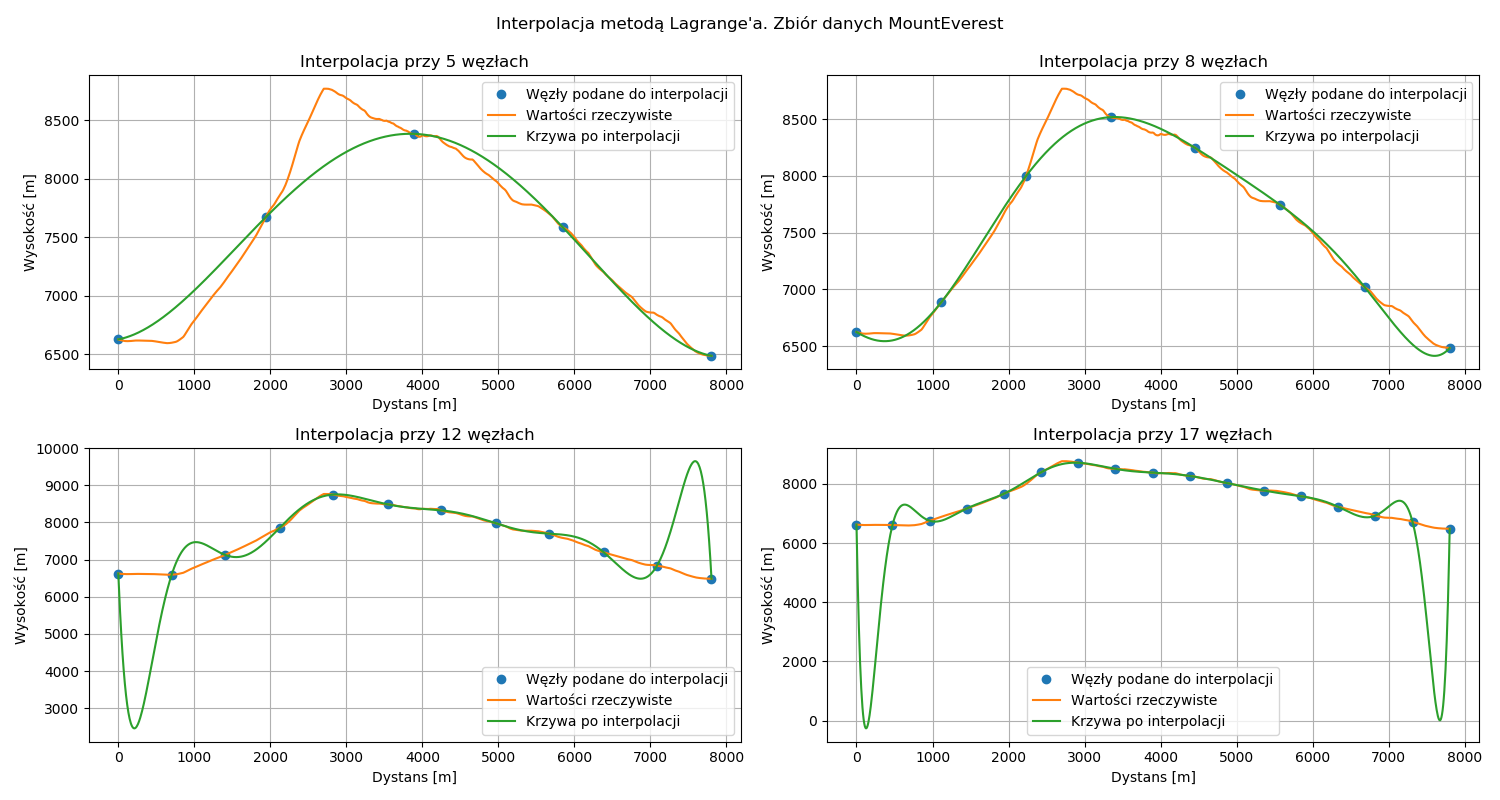
\includegraphics[scale=0.42]{../plots/lagrange_MountEverest.png}
    \caption{Wykresy interpolacji metodą Lagrange'a zbioru MountEverest}
\end{figure}
\begin{figure}[H]
    \centering
    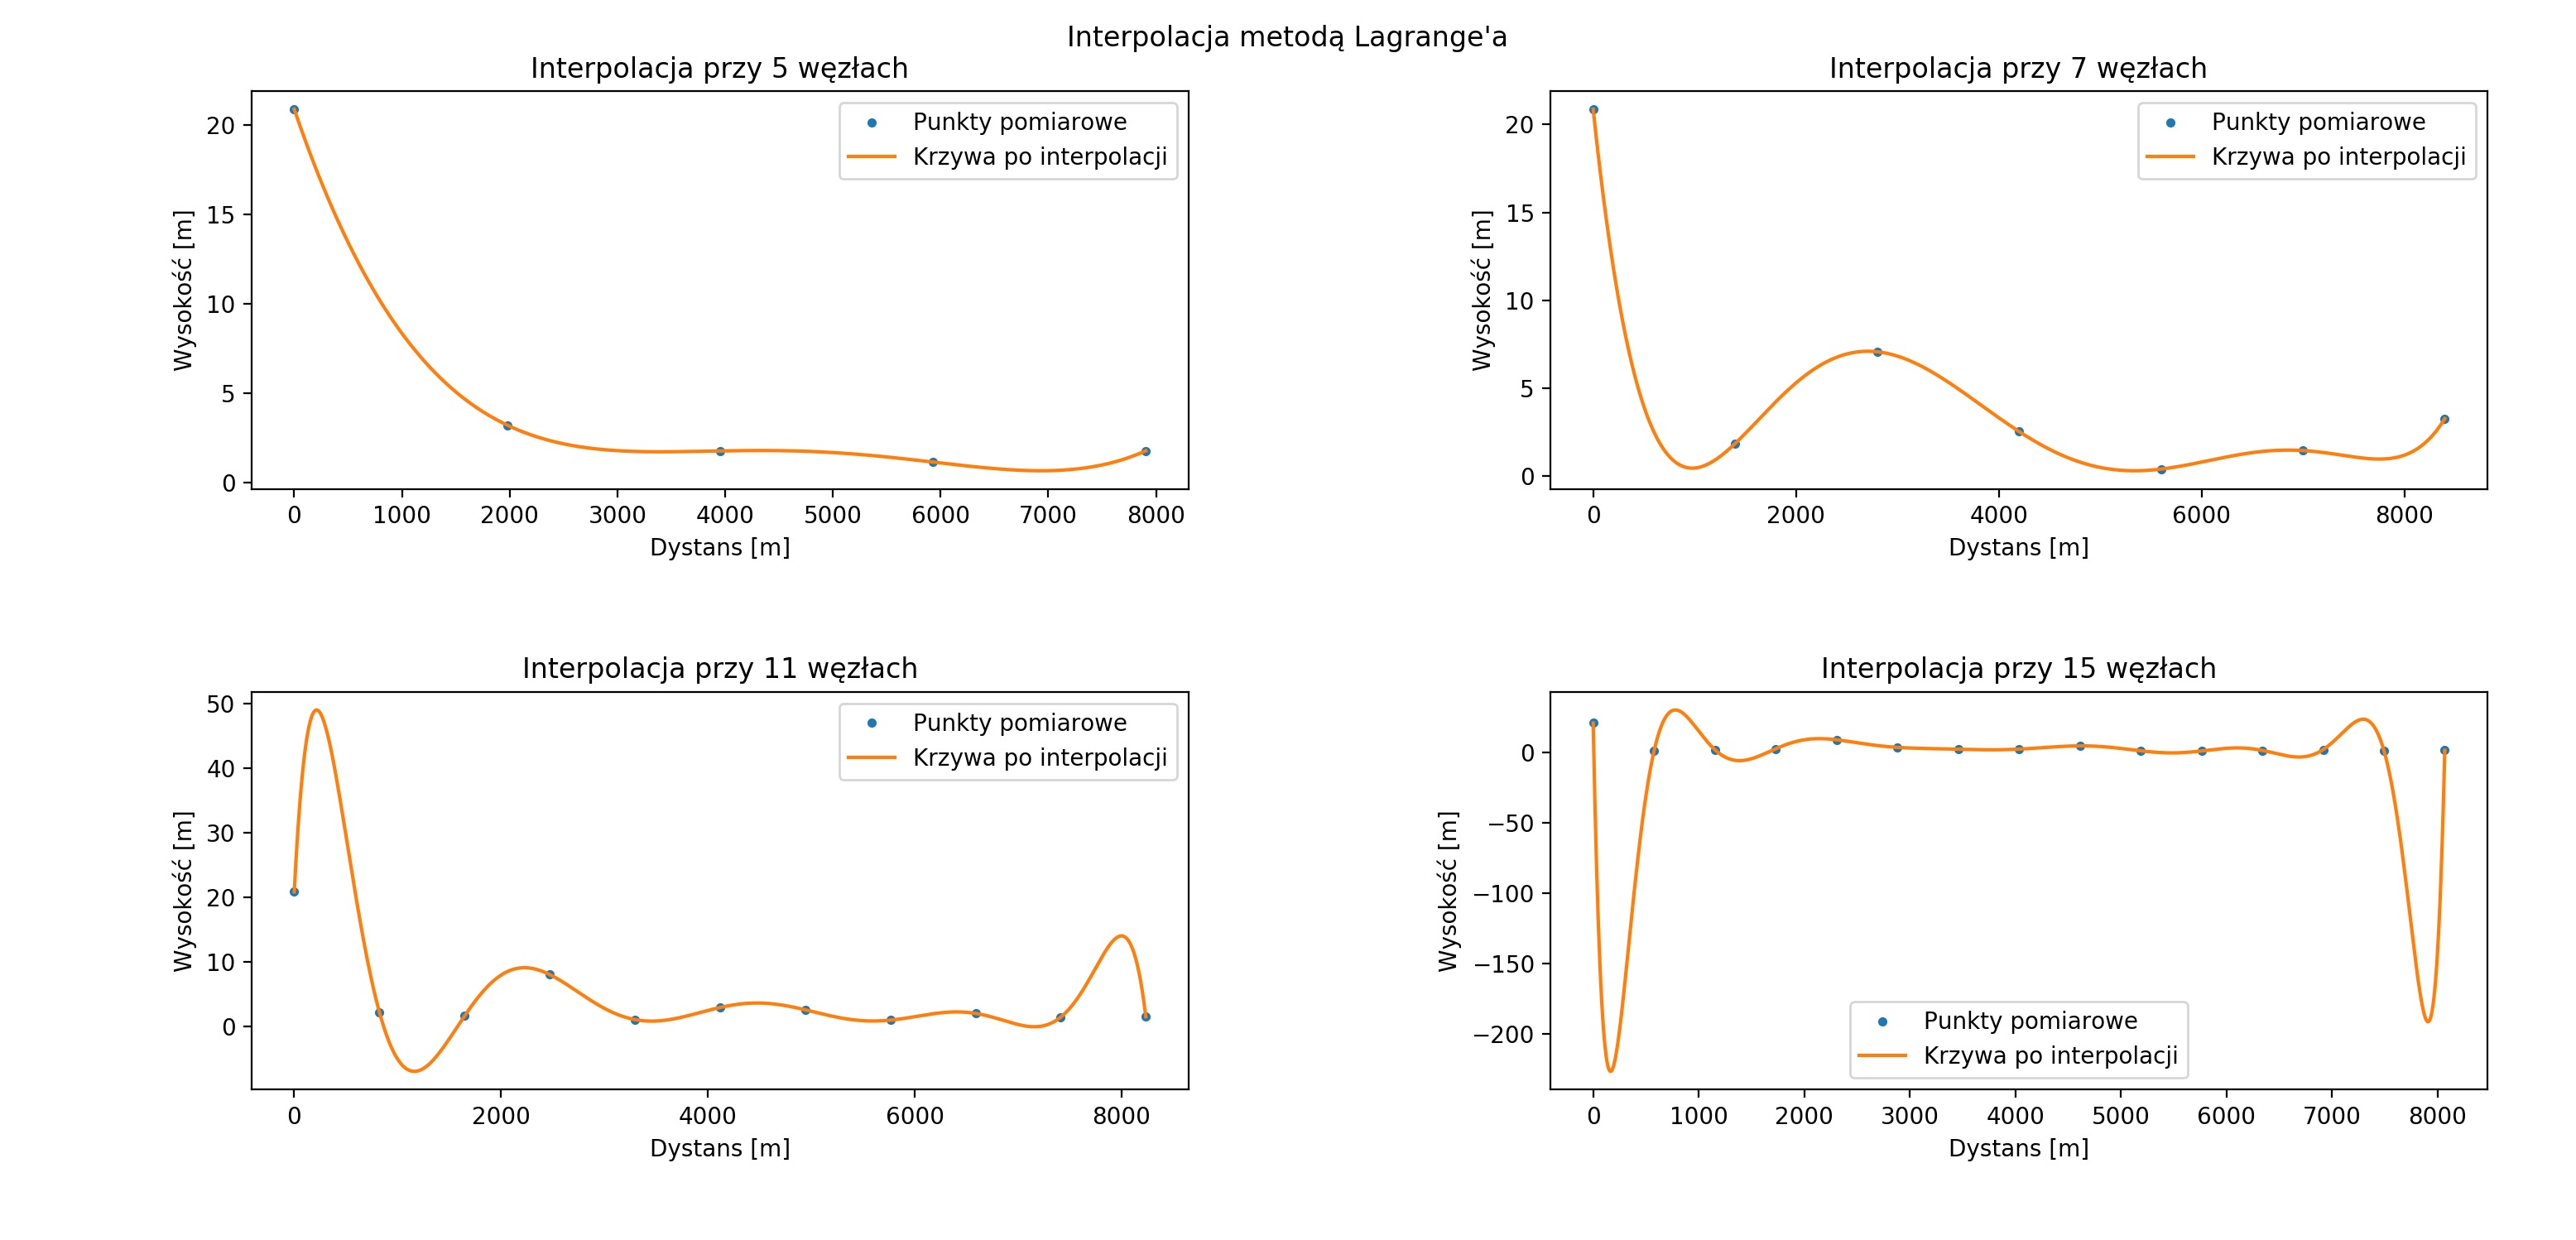
\includegraphics[scale=0.42]{../plots/lagrange_SpacerniakGdansk.png}
    \caption{Wykresy interpolacji metodą Lagrange'a zbioru SpacerniakGdansk}
\end{figure}
\begin{figure}[H]
    \centering
    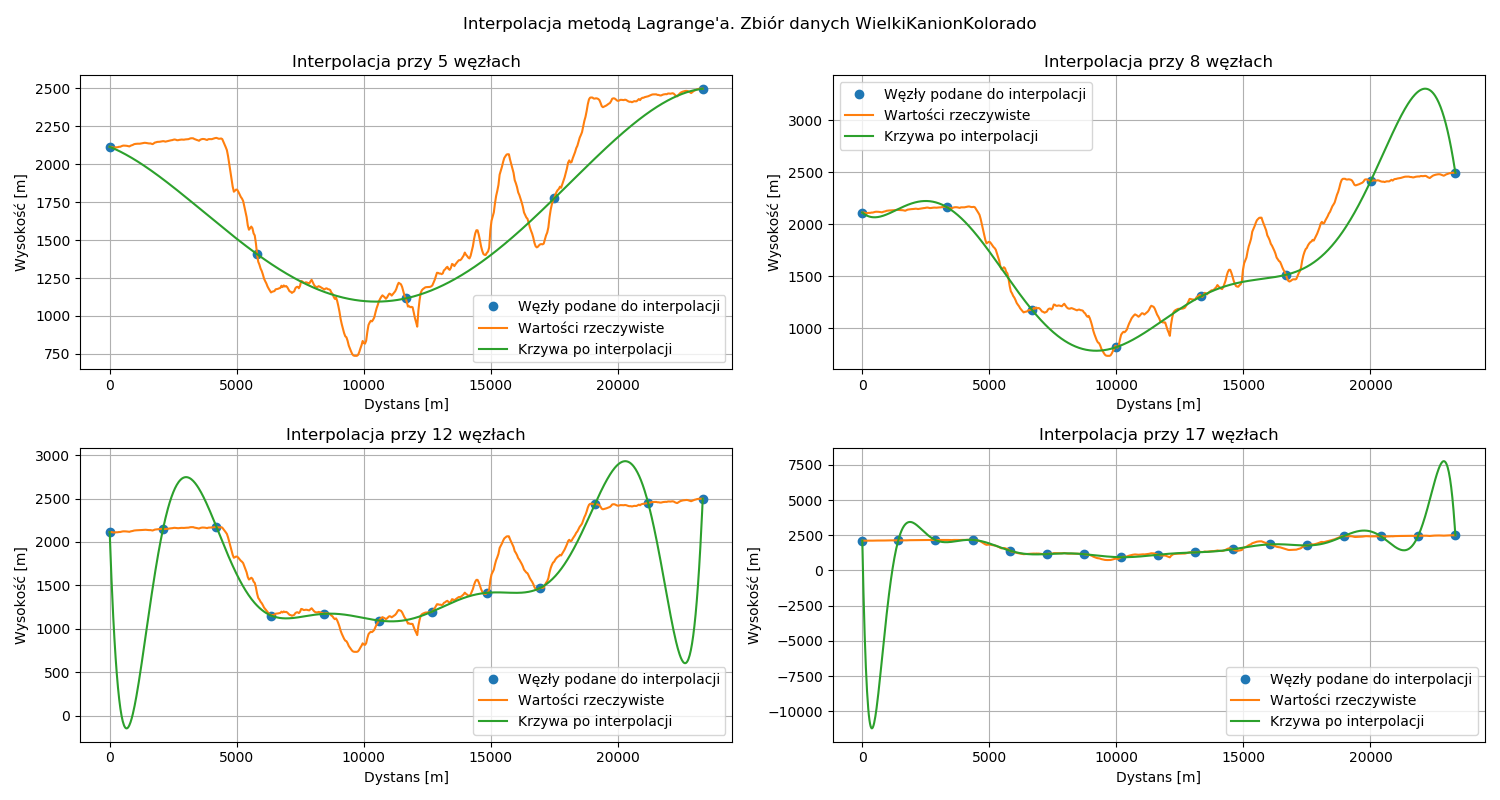
\includegraphics[scale=0.42]{../plots/lagrange_WielkiKanionKolorado.png}
    \caption{Wykresy interpolacji metodą Lagrange'a zbioru WielkiKanionKolorado}
\end{figure}
\begin{figure}[H]
    \centering
    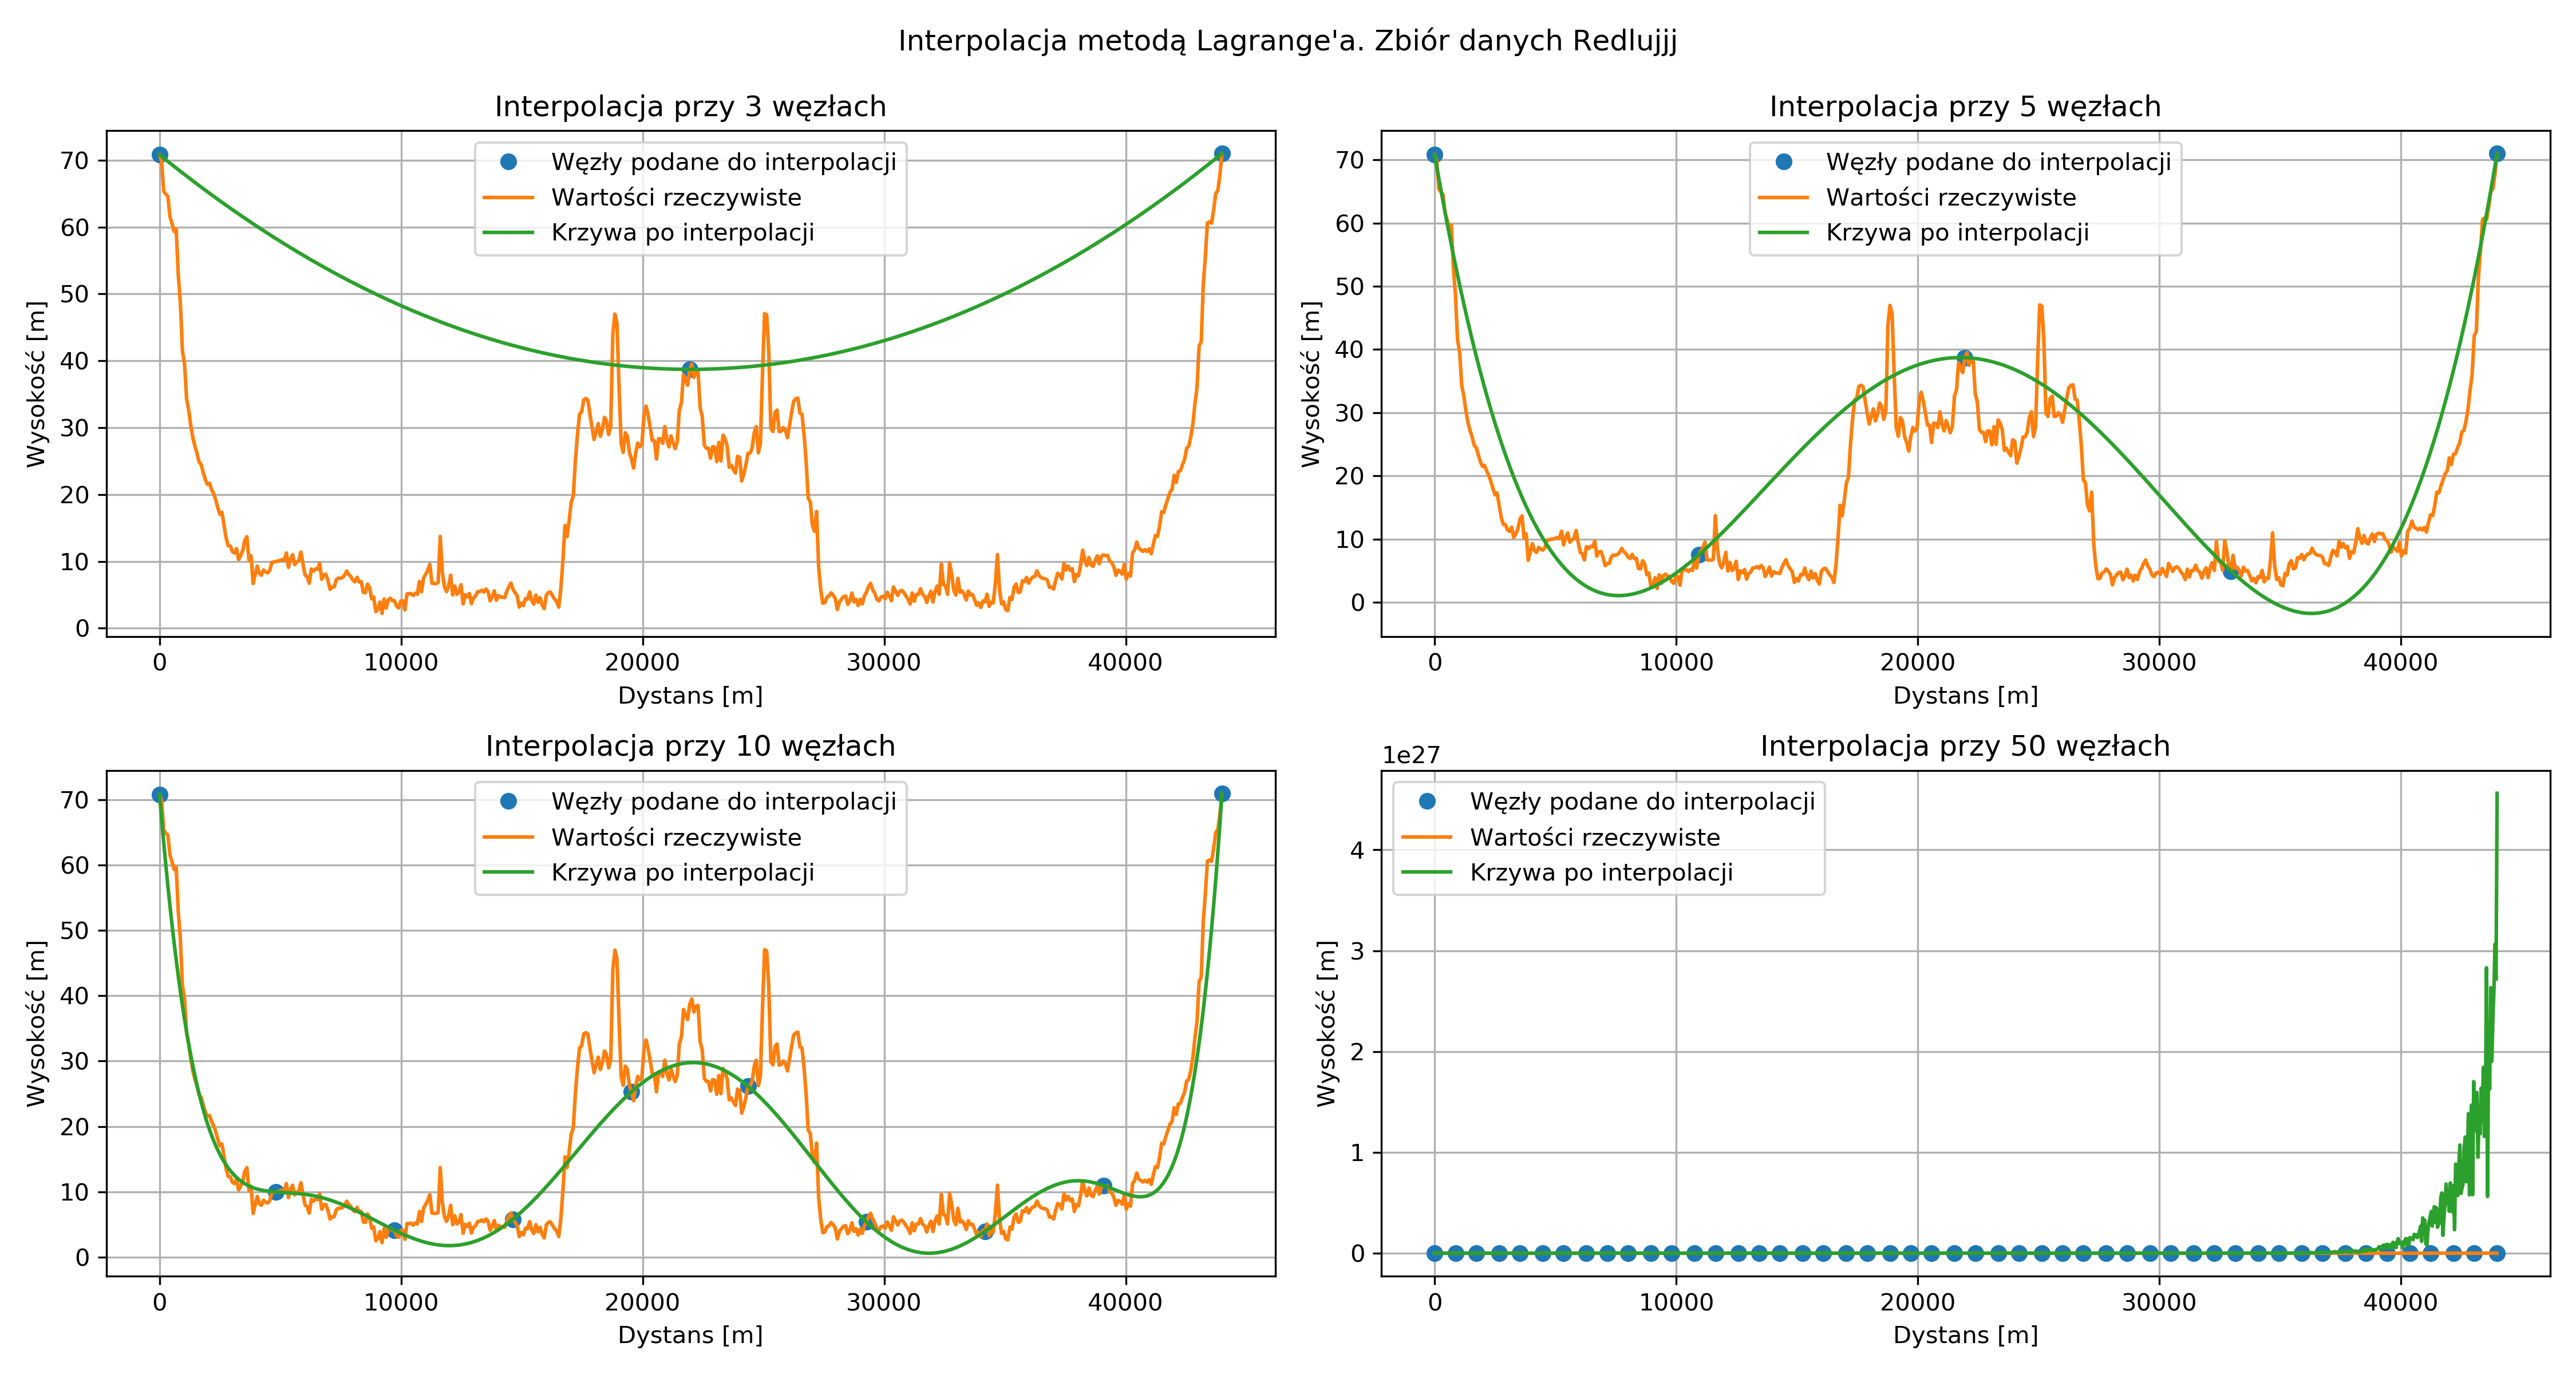
\includegraphics[scale=0.42]{../plots/lagrange_Redlujjj.png}
    \caption{Wykresy interpolacji metodą Lagrange'a zbioru Redlujjj}
\end{figure}

\subsubsection{Błąd przybliżenia funkcji wielomianem wysokiego rzędu}
Na wykresach wyraźnie widać że wielomian radzi sobie coraz lepiej z przybliżaniem wartości na środku przedziału, jednak kiedy zwiększamy ilość węzłów pomiarowych skala wykresu zostaje zdominowana przez anomalie na krańcach przedziału.
\begin{figure}[H]
    \centering
    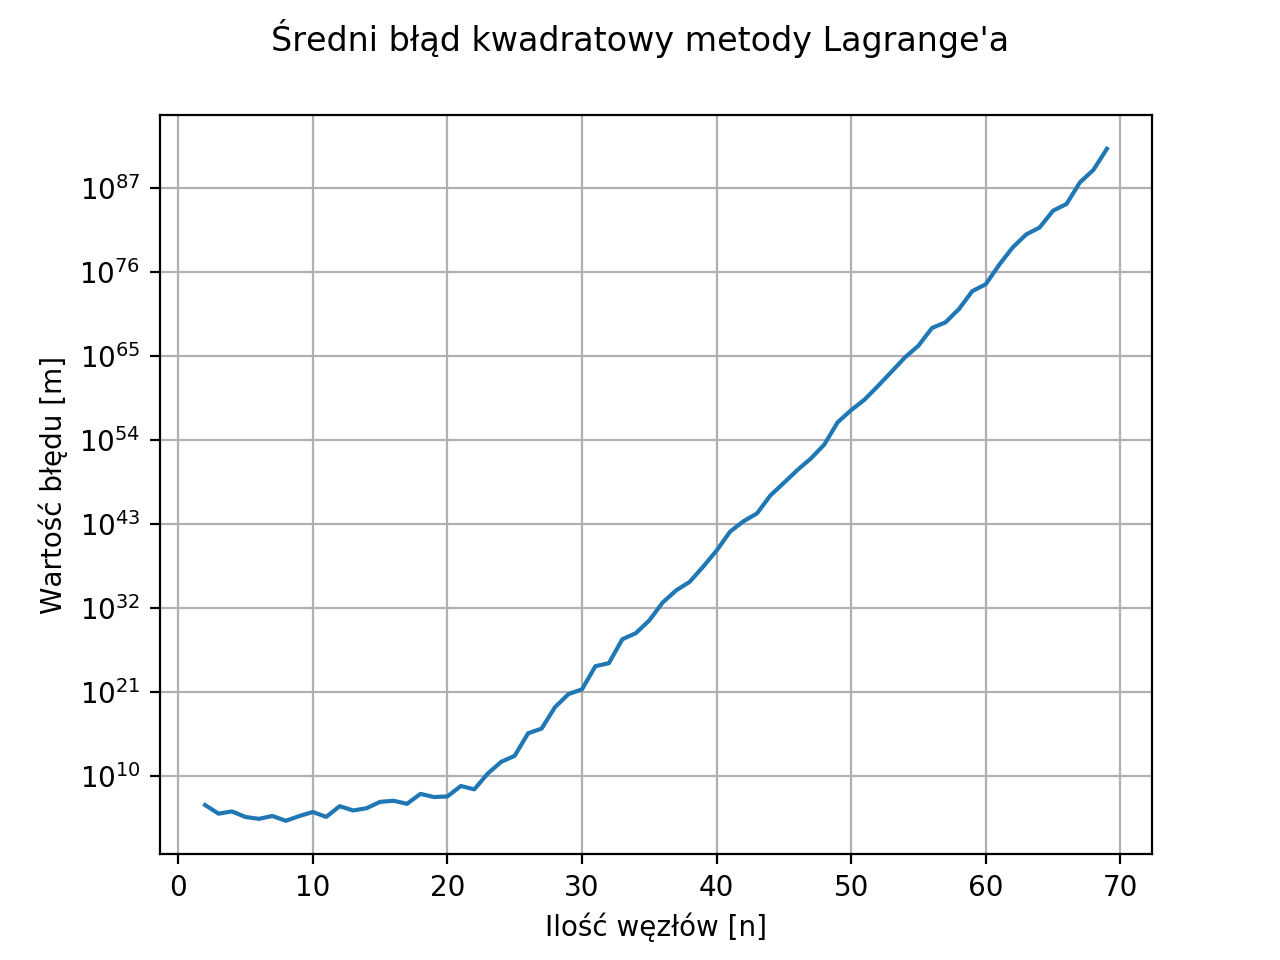
\includegraphics[scale=0.8]{../plots/error_lagrange_MountEverest.png}
    \caption{Przykładowy wykres średniego błędu kwadratowego dla metody Lagrange'a dla zbioru MountEverest}
\end{figure}
Na wykresie średniego błędu kwadratowego wyraźnie widać że zwiększanie stopnia wielomianu przez podanie większej ilości danych paradoksalnie, zamiast polepszać pogarsza wyniki.
\subsubsection{Efekt Rungego}
Oscylacje powstające na krańcach przedziałów spowodowane są efektem Rungego. Efekt ten powstaje w wyniku zastosowania do interpolacji równo odległych punktów przez które wielomian, chcąc zachować swoją ciągłość podczas przechodzenia przez węzły musi pomiędzy nimi odchylać się o bardzo duże wartości, powodując tym samym spadek dokładności aproksymacji.
\subsubsection{Wnioski}
Interpolacja zbioru punktów za pomocą wielomianu jest bardzo prostym działaniem. Zaimplementowanie tej metody w Pythonie wymagało zaledwie kilkunastu linii kodu, jednak obarczone jest to ceną w postaci dokładności. Metoda jest dosyć dokładna w środku przedziału dlatego w oparciu o estymator optymalnej ilości węzłów jest w stanie z niską dokładnością przybliżać wartości funkcji ze środka przedziału.
\subsection{Metoda funkcji sklejanych, splajnów (ang. splines)}
Aby zniwelować błędy spowodowane interpolacją globalną, tj. w przypadku interpolacji wielomianowej, lepiej jest wyznaczyć wielomian niskiego stopnia dla danego podprzedziału.\\
Metoda funkcji sklejanych polega na wyznaczeniu dla \(n+1\) węzłów pomiarowych \(n\) wielomianów \(S_i(x)\), które odpowiadają wartościom interpolowanej krzywej w przedziale \(\left<x_i, x_{i+1}\right)\). do tego celu najlepiej sprawdzają się wielomiany minimum 3 stopnia, niższe nie mogą przechować wystarczająco dużo informacji potrzebnych do zadowalającego wyniku.
\subsubsection{Wymagania dla funkcji sklejanych}
Ze względu na wykorzystanie \(n\) funkcji zamiast jednej konieczne jest wymuszenie warunków na każdym z wielomianów:
\begin{itemize}
    \item wielomian \(S_i(x)\) musi sie równać wartościom funkcji na krańcach przedziału \(\rightarrow S_i(x_i) = f(x_i) \wedge S_i(x_{i+1}) = f(x_{i+1})\)
    \item dwa wielomiany muszą być ciągłe w punkcie złączenia \(\rightarrow S_i'(x_i) = S_{i+1}'(x_i)\)
    \item aby uniknąć oscylującej wklęsłości/wypukłości \(\rightarrow S_i''(x_i) = S_{i+1}''(x_i)\)
    \item do określenia układu równań potrzebne są jeszcze 2 równania więc spowodujmy wypłaszczenie funkcji na krańcach zbiorów  \(\rightarrow S_0''(x_0) = 0 \wedge S_n''(x_n) = 0\)
\end{itemize}
Rozwiązując powyższe rówania, otrzymujemy współczynniki \(n\) wielomianów.
\subsubsection{Dokładność dopasowania funkcji sklejanych w zależności od ilości węzłów}
\begin{figure}[H]
    \centering
    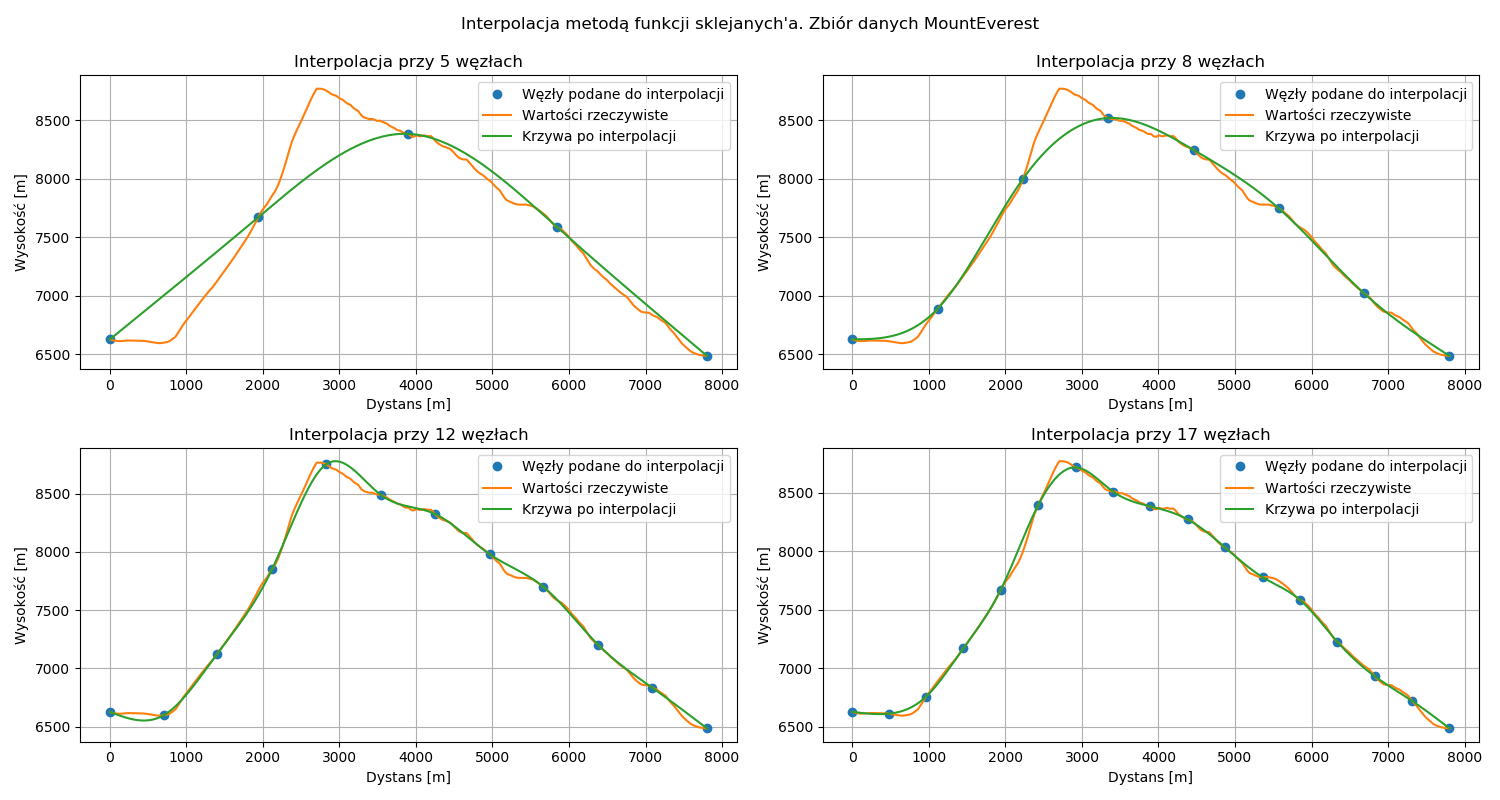
\includegraphics[scale=0.47]{../plots/splines_MountEverest.png}
    \caption{Wykresy interpolacji zbioru MountEverest metodą funkcji sklejanych}
\end{figure}
\begin{figure}[H]
    \centering
    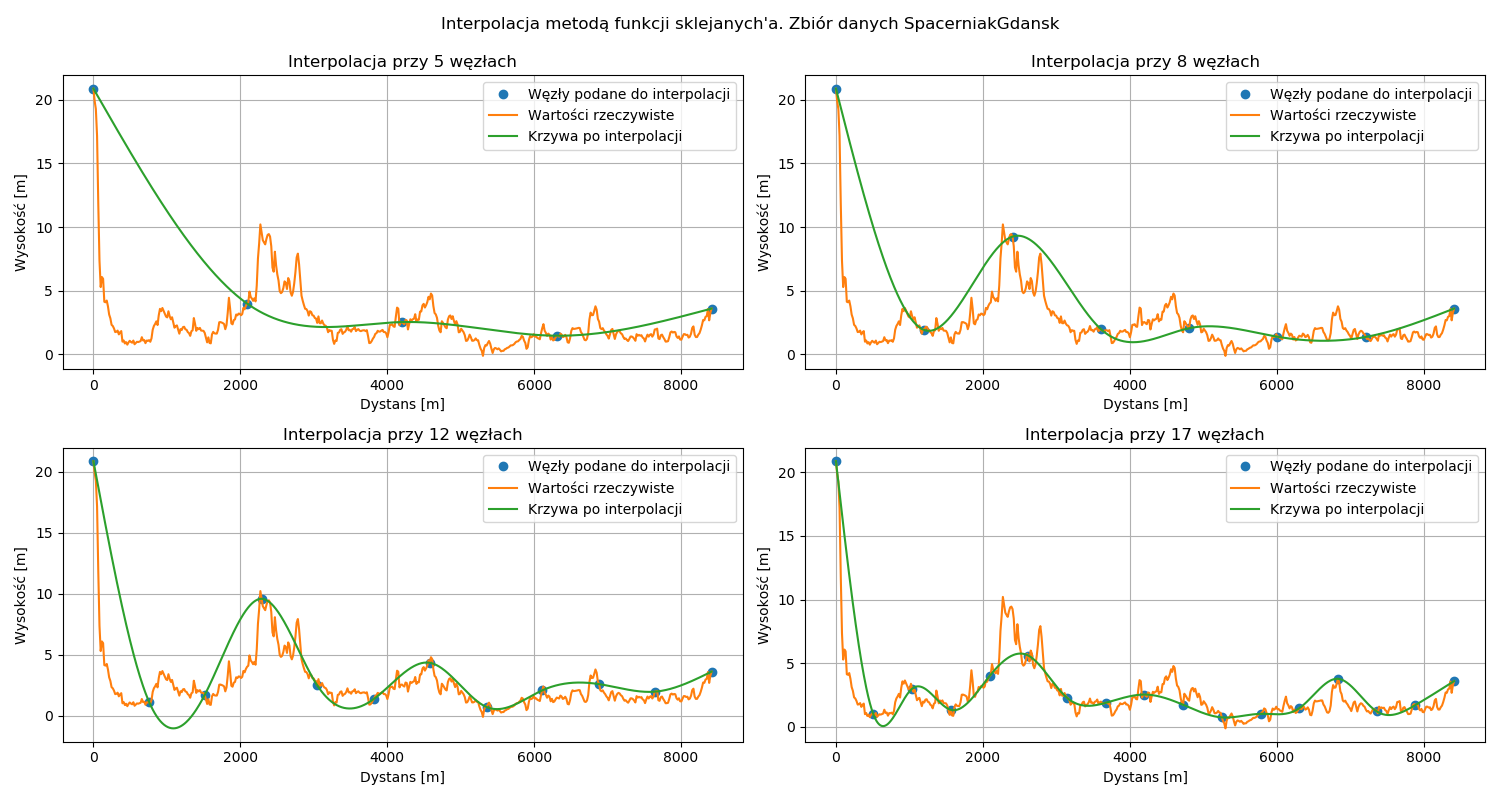
\includegraphics[scale=0.47]{../plots/splines_SpacerniakGdansk.png}
    \caption{Wykresy interpolacji zbioru SpacerniakGdansk metodą funkcji sklejanych}    
\end{figure}
\begin{figure}[H]
    \centering
    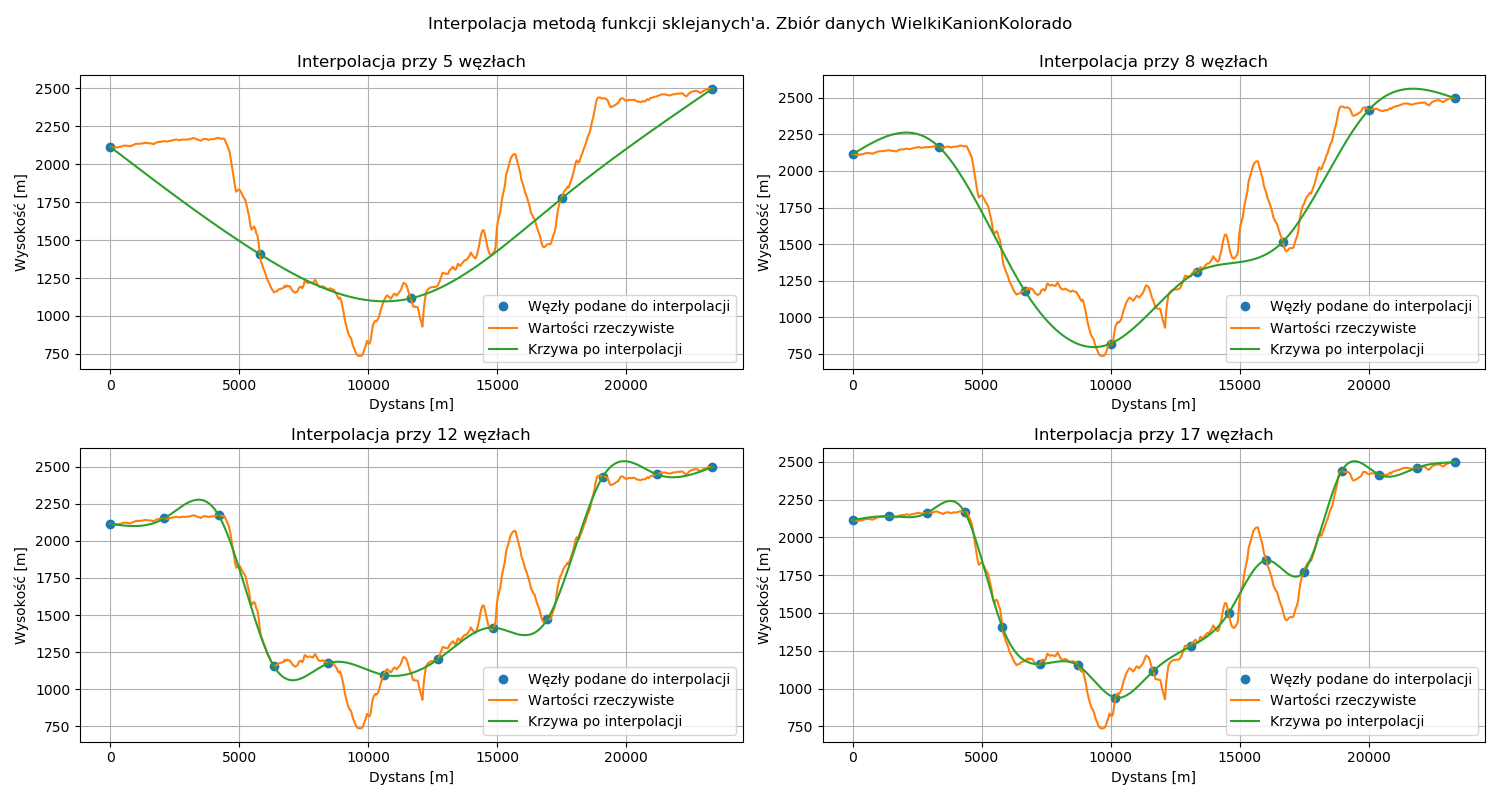
\includegraphics[scale=0.47]{../plots/splines_WielkiKanionKolorado.png}
    \caption{Wykresy interpolacji zbioru WielkiKanionKolorado}    
\end{figure}
\begin{figure}[H]
    \centering
    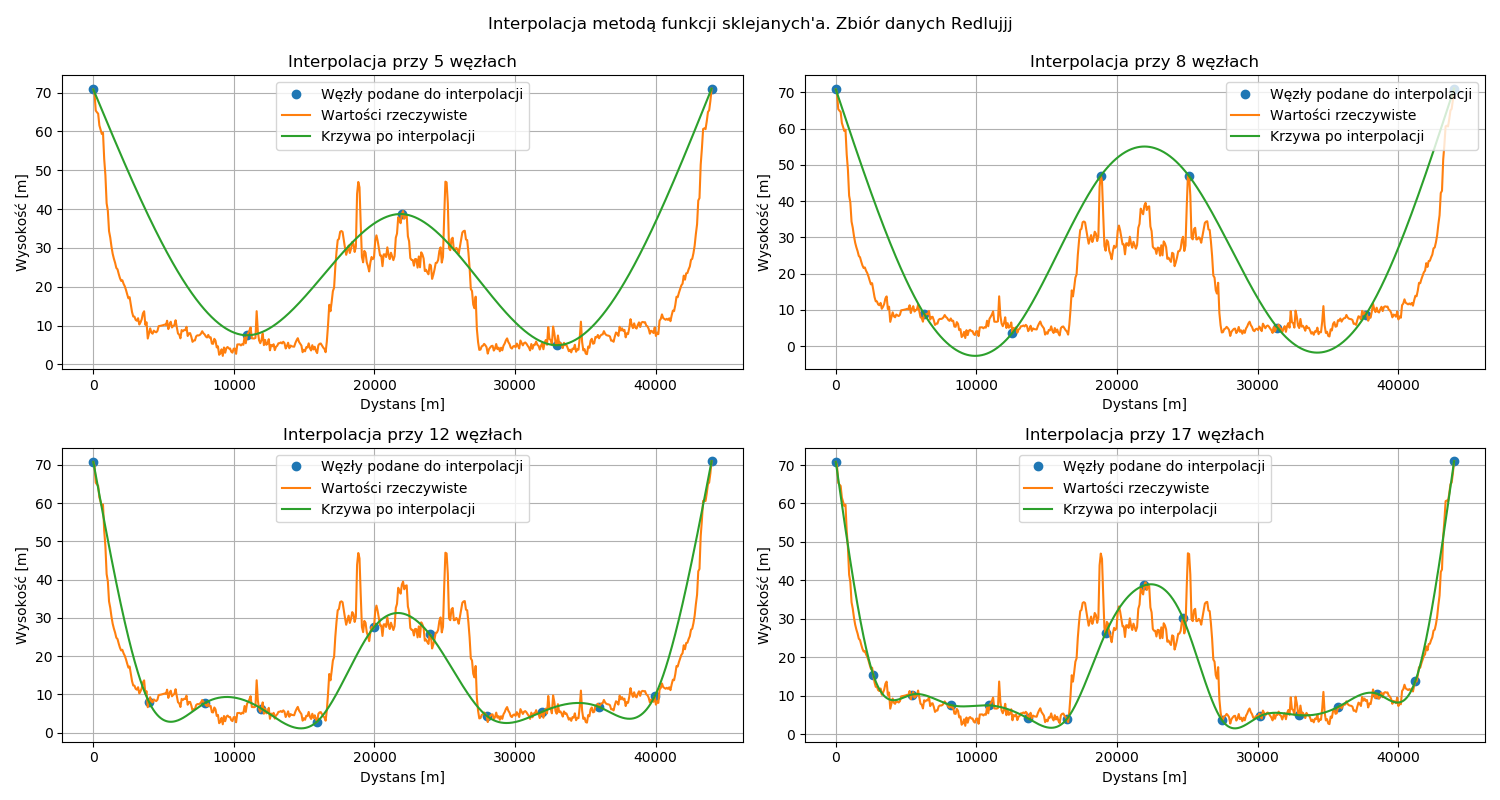
\includegraphics[scale=0.47]{../plots/splines_Redlujjj.png}
    \caption{Wykresy interpolacji zbioru Redlujjj metodą funkcji sklejanych}
\end{figure}

\subsubsection{Błąd interpolacji metodą funkcji sklejanych}
Na pierwszy rzut oka widać, że metoda splajnów jest znacznie dokładniejsza. Nie występuje tutaj efekt Rungego, a każdy z wielomianów bardzo dobrze opisuje wykres lokalnie.
\begin{figure}[H]
   \centering
   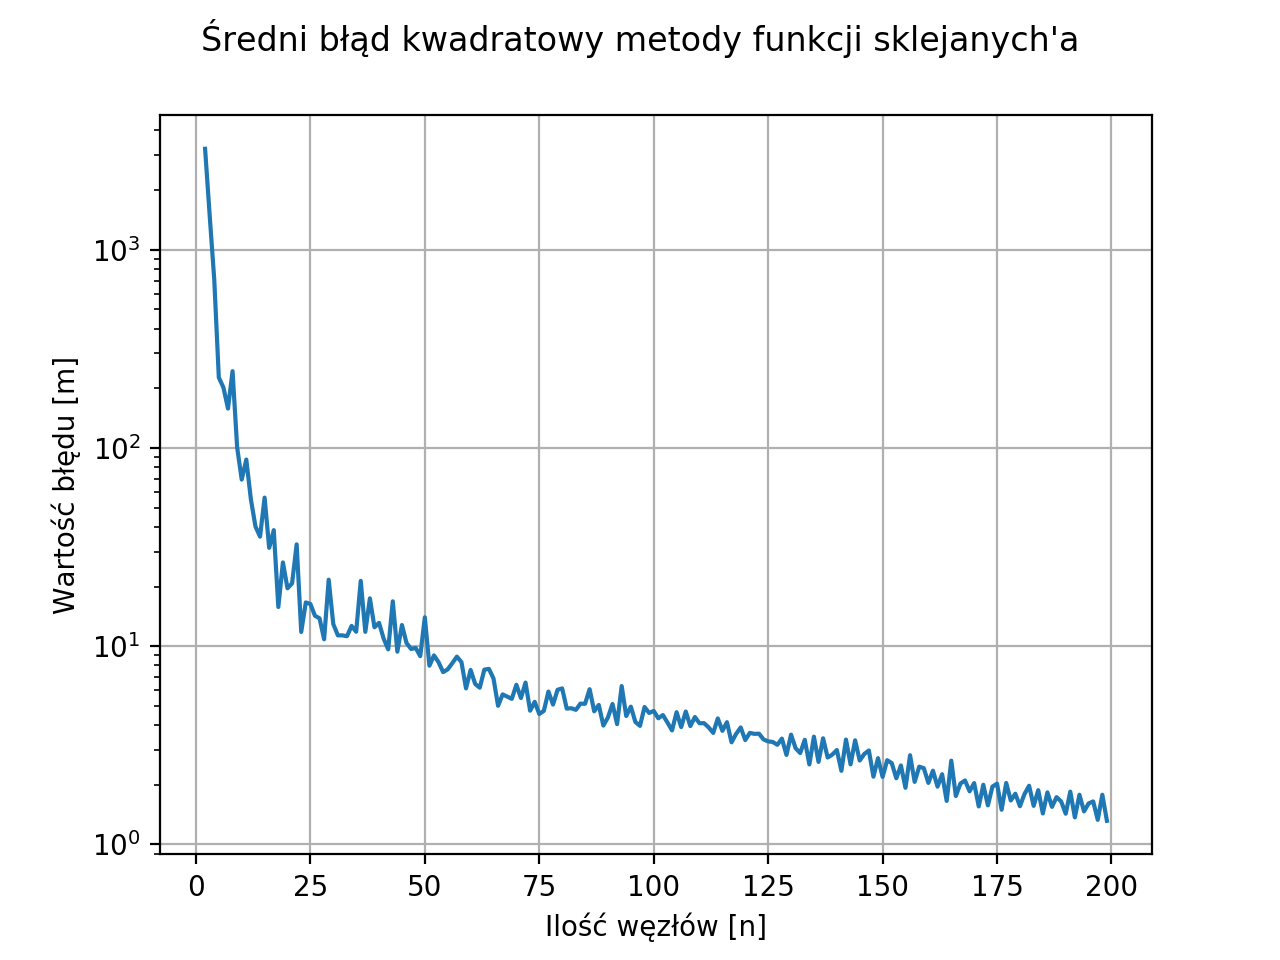
\includegraphics[scale=0.7]{../plots/error_splines_Redlujjj.png}
   \caption{Wykres średniego błędu kwadratowego interpolacji metodą funkcji sklejanych dla zbioru Redlujj} 
\end{figure}
Patrząc na wykres błedu, można pokusić się o stwierdzenie, że zwiększanie liczby węzłów sukcesywnie zwiększa dokładność interpolacji, co potwierdza poniższy wykres.
\begin{figure}[H]
    \centering
    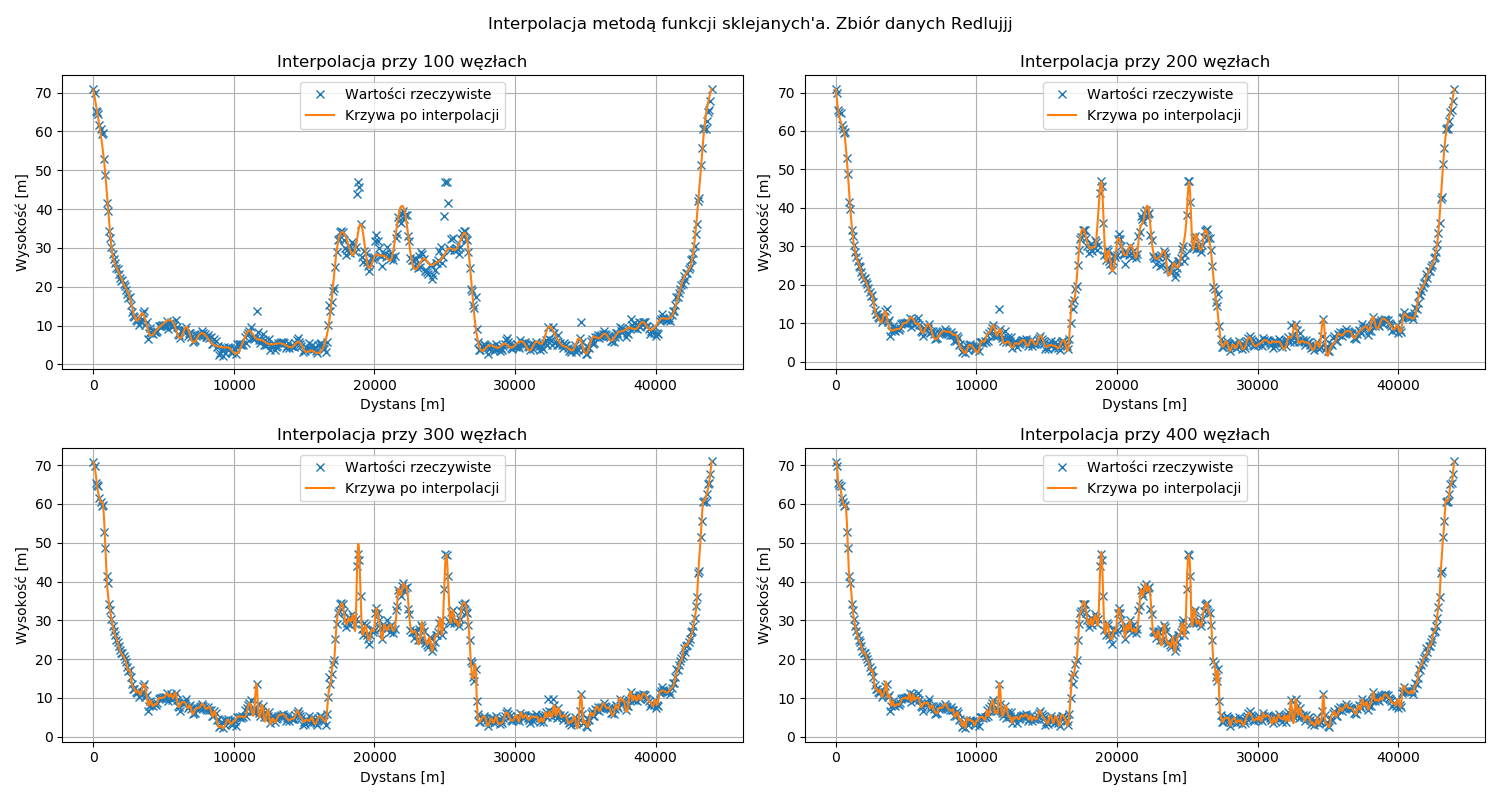
\includegraphics[scale=0.5]{../plots/splines_accurate_Redlujjj.png}
    \caption{Wykres interpolacji zbioru Redlujj przy pomocy funkcji sklejanych i wysokiej ilości węzłów}
\end{figure}
\subsubsection{Wnioski}
Metoda funkcji sklejanych jest bardzo dobrą metodą do interpolacji dowolnego zbioru danych, ze względu na to że zbiór jest interpolowany lokalnie, więc każda z funkcji bazowych może się skupić na wartościach w tym przedziale, pod warunkiem, że spełni wymagania postawione na początku (ciągłość i wypukłość). W odróżnieniu od interpolacji wielomianowej, funkcje sklejane pozwalają na użycie calego zbioru dostępnych danych, dzięki czemu możemy uzyskać nowe dokładne wartości w podprzedziałach, wykorzystując całkowicie wiedzę zdobytą wcześniej.
\section{Podsumowanie}
Interpolacja to bardzo ciekawy i wysoce satysfakcjonujący w implementacji temat. Kiedy posiadamy wystarczająco dokładne pomiary, jesteśmy w stanie wyznaczyć dowolną ciągłą krzywą, bez konieczności wyrażania jej konkretnym wzorem, co jest bardzo pomocne, jeśli takie działanie jest trudne lub wręcz niemożliwe. Interpolacja wielomianowa jest bardzo prymitywnym sposobem, który jest prosty w implementacji, jednak kiepsko sprawdza się w praktyce, głównie przez efekt Rungego. Być może wada ta byłaby mniej widoczna jeśli węzły mierzone byłyby niejednostajnie, jednak generuje to nowy problem określenia, który węzeł jest lepszy od drugiego. Metoda funkcji sklejanych natomiast sprawdza się doskonale praktycznie na każdym zbiorze danych, ponieważ pozwala na wykorzystanie całego dostępnego zbioru węzłów.


\end{document}
